\documentclass[12pt]{article}

\usepackage[utf8]{inputenc}
\usepackage{amssymb}
\usepackage{amsfonts}
\usepackage{amsmath}
\usepackage{graphicx}
\usepackage[margin=1in]{geometry}
\usepackage[hidelinks]{hyperref}
\usepackage{float}
\usepackage[danish]{varioref}
\usepackage{multirow}
\usepackage{hhline}
\usepackage{inconsolata}
\usepackage{etoolbox}
\usepackage[usenames,dvipsnames]{xcolor}
\usepackage{tikz}
\usetikzlibrary{positioning,shapes, shadows, arrows}
\usepackage{listings}

\definecolor{dark-blue}{HTML}{000080}
\definecolor{dark-green}{HTML}{008000}
\definecolor{pale-purple}{HTML}{94558D}
\definecolor{dark-purple}{HTML}{0000AA}
\definecolor{regular-purple}{HTML}{660099}
\definecolor{magenta}{HTML}{B200B2}
\definecolor{light-gray}{HTML}{FAFAFA}
\definecolor{dark-gray}{HTML}{2D2D2D}
\definecolor{comment}{HTML}{808080}
\definecolor{digit}{HTML}{0000FF}

\newcommand*{\FormatDigit}[1]{\textcolor{digit}{#1}}

\lstset{
	language=Python,
	prebreak=\raisebox{0ex}[0ex][0ex]{\ensuremath{\color{red}\space\hookleftarrow}},
	basicstyle=\footnotesize\ttfamily,
	%
	literate=%
    	{0}{{\FormatDigit{0}}}{1}%
        {1}{{\FormatDigit{1}}}{1}%
        {2}{{\FormatDigit{2}}}{1}%
        {3}{{\FormatDigit{3}}}{1}%
        {4}{{\FormatDigit{4}}}{1}%
        {5}{{\FormatDigit{5}}}{1}%
        {6}{{\FormatDigit{6}}}{1}%
        {7}{{\FormatDigit{7}}}{1}%
        {8}{{\FormatDigit{8}}}{1}%
        {9}{{\FormatDigit{9}}}{1}%
        {.0}{{\FormatDigit{.0}}}{2}% Following is to ensure that only periods
        {.1}{{\FormatDigit{.1}}}{2}% followed by a digit are changed.
        {.2}{{\FormatDigit{.2}}}{2}%
        {.3}{{\FormatDigit{.3}}}{2}%
        {.4}{{\FormatDigit{.4}}}{2}%
        {.5}{{\FormatDigit{.5}}}{2}%
        {.6}{{\FormatDigit{.6}}}{2}%
        {.7}{{\FormatDigit{.7}}}{2}%
        {.8}{{\FormatDigit{.8}}}{2}%
        {.9}{{\FormatDigit{.9}}}{2}%
        %{,}{{\FormatDigit{,}}{1}% depends if you want the "," in color
        {\ }{{ }}{1}% handle the space
		{æ}{{\ae}}1
        {ø}{{\o}}1
        {å}{{\aa}}1
        {Æ}{{\AE}}1	
        {Ø}{{\O}}1
        {Å}{{\AA}}1,
	%
	%emph={},
	otherkeywords={},
	keywords=[2]{self},
	keywords=[3]{__init__},
	keywords=[4]{object},
	keywords=[5]{encoding, flags},
	keywords=[6]{reduce,list,enumerate,len,map,range,sorted,None,super,@staticmethod},
	%
	keywordstyle=\bfseries\color{dark-blue},
	keywordstyle={[2]\color{pale-purple}},
	keywordstyle={[3]\color{magenta}},
	keywordstyle={[4]\color{dark-blue}},
	keywordstyle={[5]\color{regular-purple}},
	keywordstyle={[6]\color{dark-purple}},
    commentstyle=\itshape\color{comment},
    identifierstyle=\color{black},
	stringstyle=\bfseries\color{dark-green},
	%emphstyle=\color{dark-purple},
	%
	numbers=left, % where to put the line-numbers
	numberstyle=\ttfamily\color{dark-gray},
	numbersep=5pt, % how far the line-numbers are from the code
	stepnumber=1,
	showstringspaces=false,
	backgroundcolor=\color{light-gray},
	tabsize=4,
	captionpos=b, % sets the caption-position to bottom
	breaklines=true % sets automatic line breaking
}

\linespread{1.3}

\begin{document}

\begin{titlepage}
    \vspace*{\fill}
    \begin{center}
      {\Huge Statistical Methods for Machine Learning}\\[0.7cm]
      {\Large Exam}\\[0.4cm]
      {\large Troels Thomsen - qvw203}\\[0.4cm]
      {\small 6. April 2015}\\[0.3cm] 
      {\small Department of Computer Science}\\
      {\small University of Copenhagen}
    \end{center}
    \vspace*{\fill}
\end{titlepage}

\clearpage

\thispagestyle{empty}

\newpage

\tableofcontents

\thispagestyle{empty}

\newpage

\setcounter{page}{1}

\section{Photometric Redshift Estimation}

\subsection{Question 1 - Linear Regression}

For linear regression we decided to use both the Maximum Likelyhood approach (ML), the Maximum A Posteriori approach (MAP), and Support Vector Regression (SVR) with a linear kernel. \\
For ML and MAP we used our own implementation from the course exercises, but for SVR we used the python Sci-kit machine learning library\footnote{\url{http://scikit-learn.org/}}. \\

\noindent To determine the best model, we compare the results for each model, using the mean-squared-error (MSE).\\
From the following test results we conclude that the model which fits our data best is Maximum Likelyhood, since we could not find an $\alpha$ which provided a smaller MSE for Maximum A Posteriori, thus yielding MAP only as good as ML.

\begin{figure}[H]
	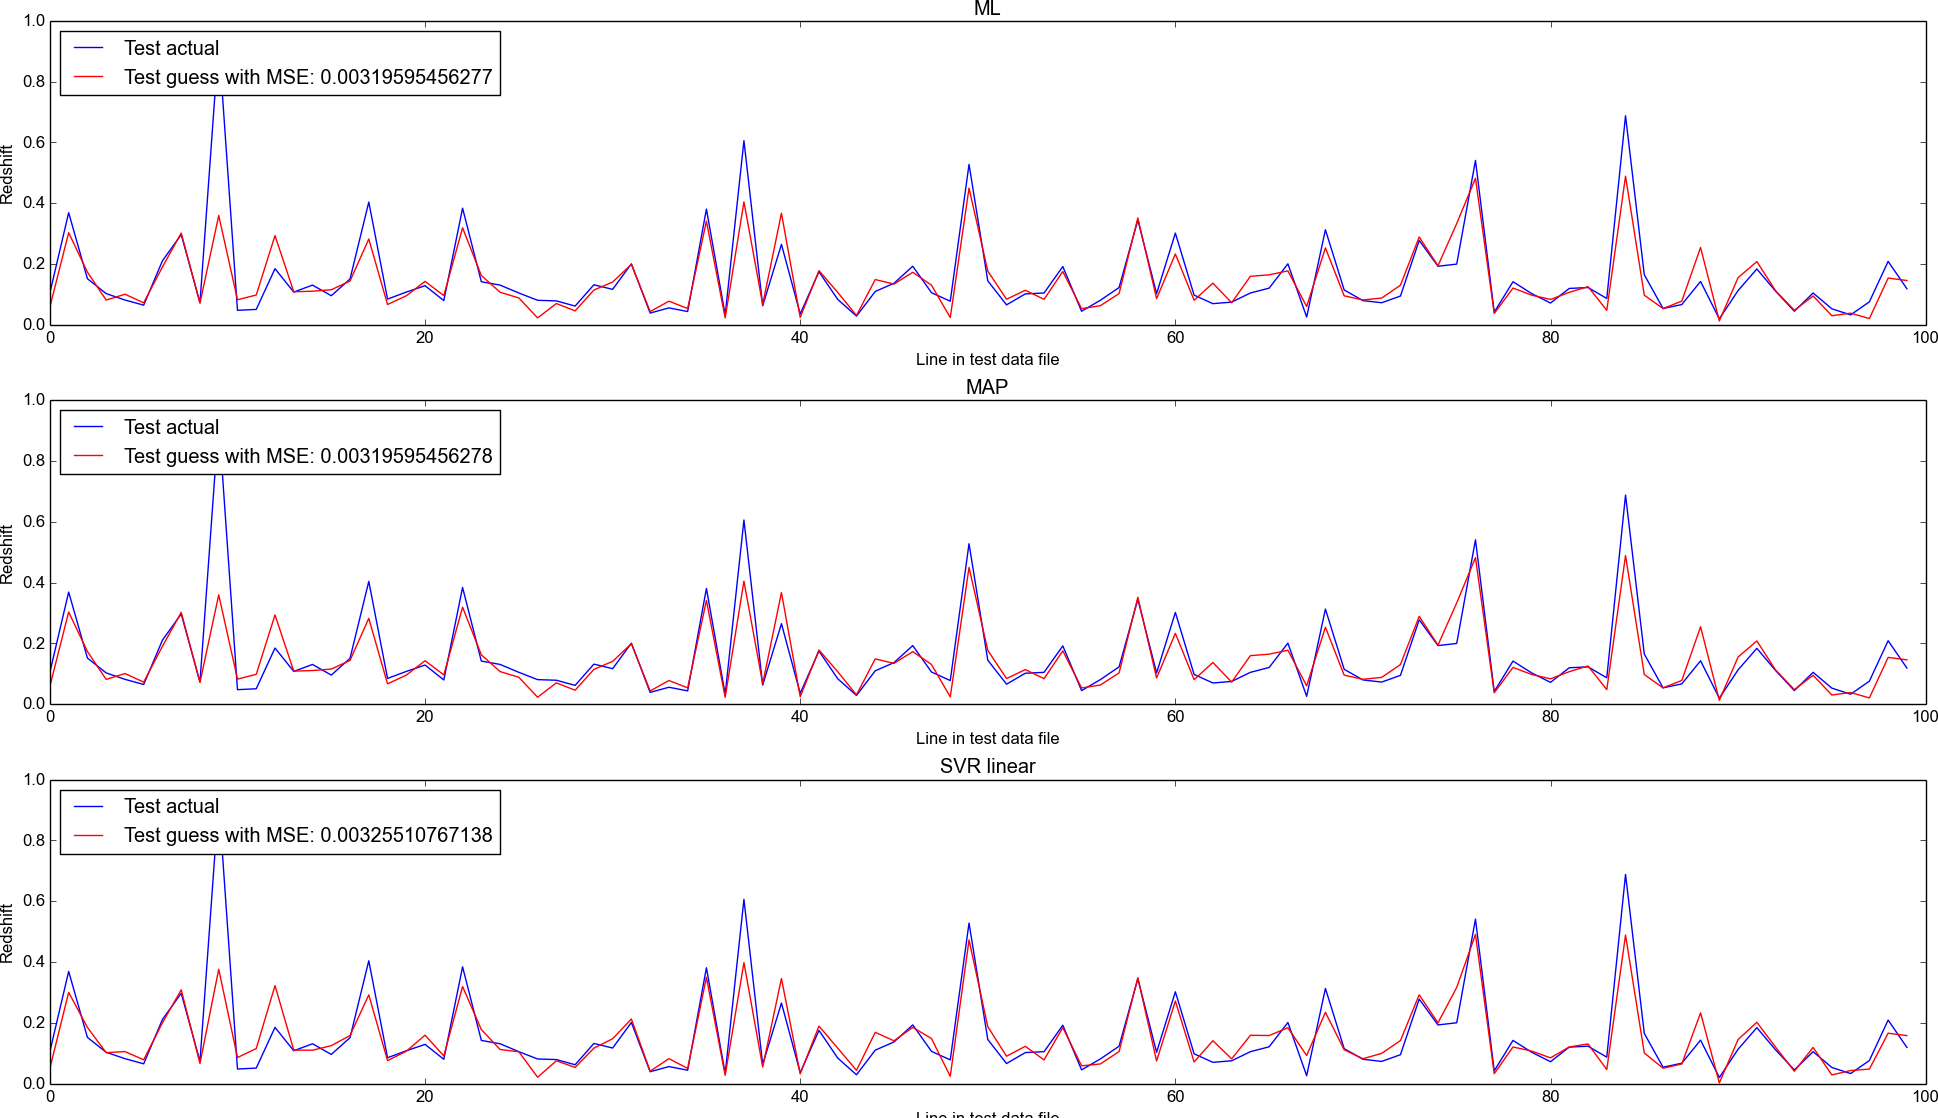
\includegraphics[scale=0.35]{linear_model.png}
	\caption{Chosen linear models - ML (Top), MAP (Middle), SVR Linear Kernel (Bottom).}
	\label{fig:linear_regression}
\end{figure}

\newpage

\subsubsection{ML results}

\begin{itemize}
	\item Training mean-squared error: $0.00281098722063$ 
	\item Test mean-squared error: $0.00319595456277$
\end{itemize}

%\begin{figure}[H]
%	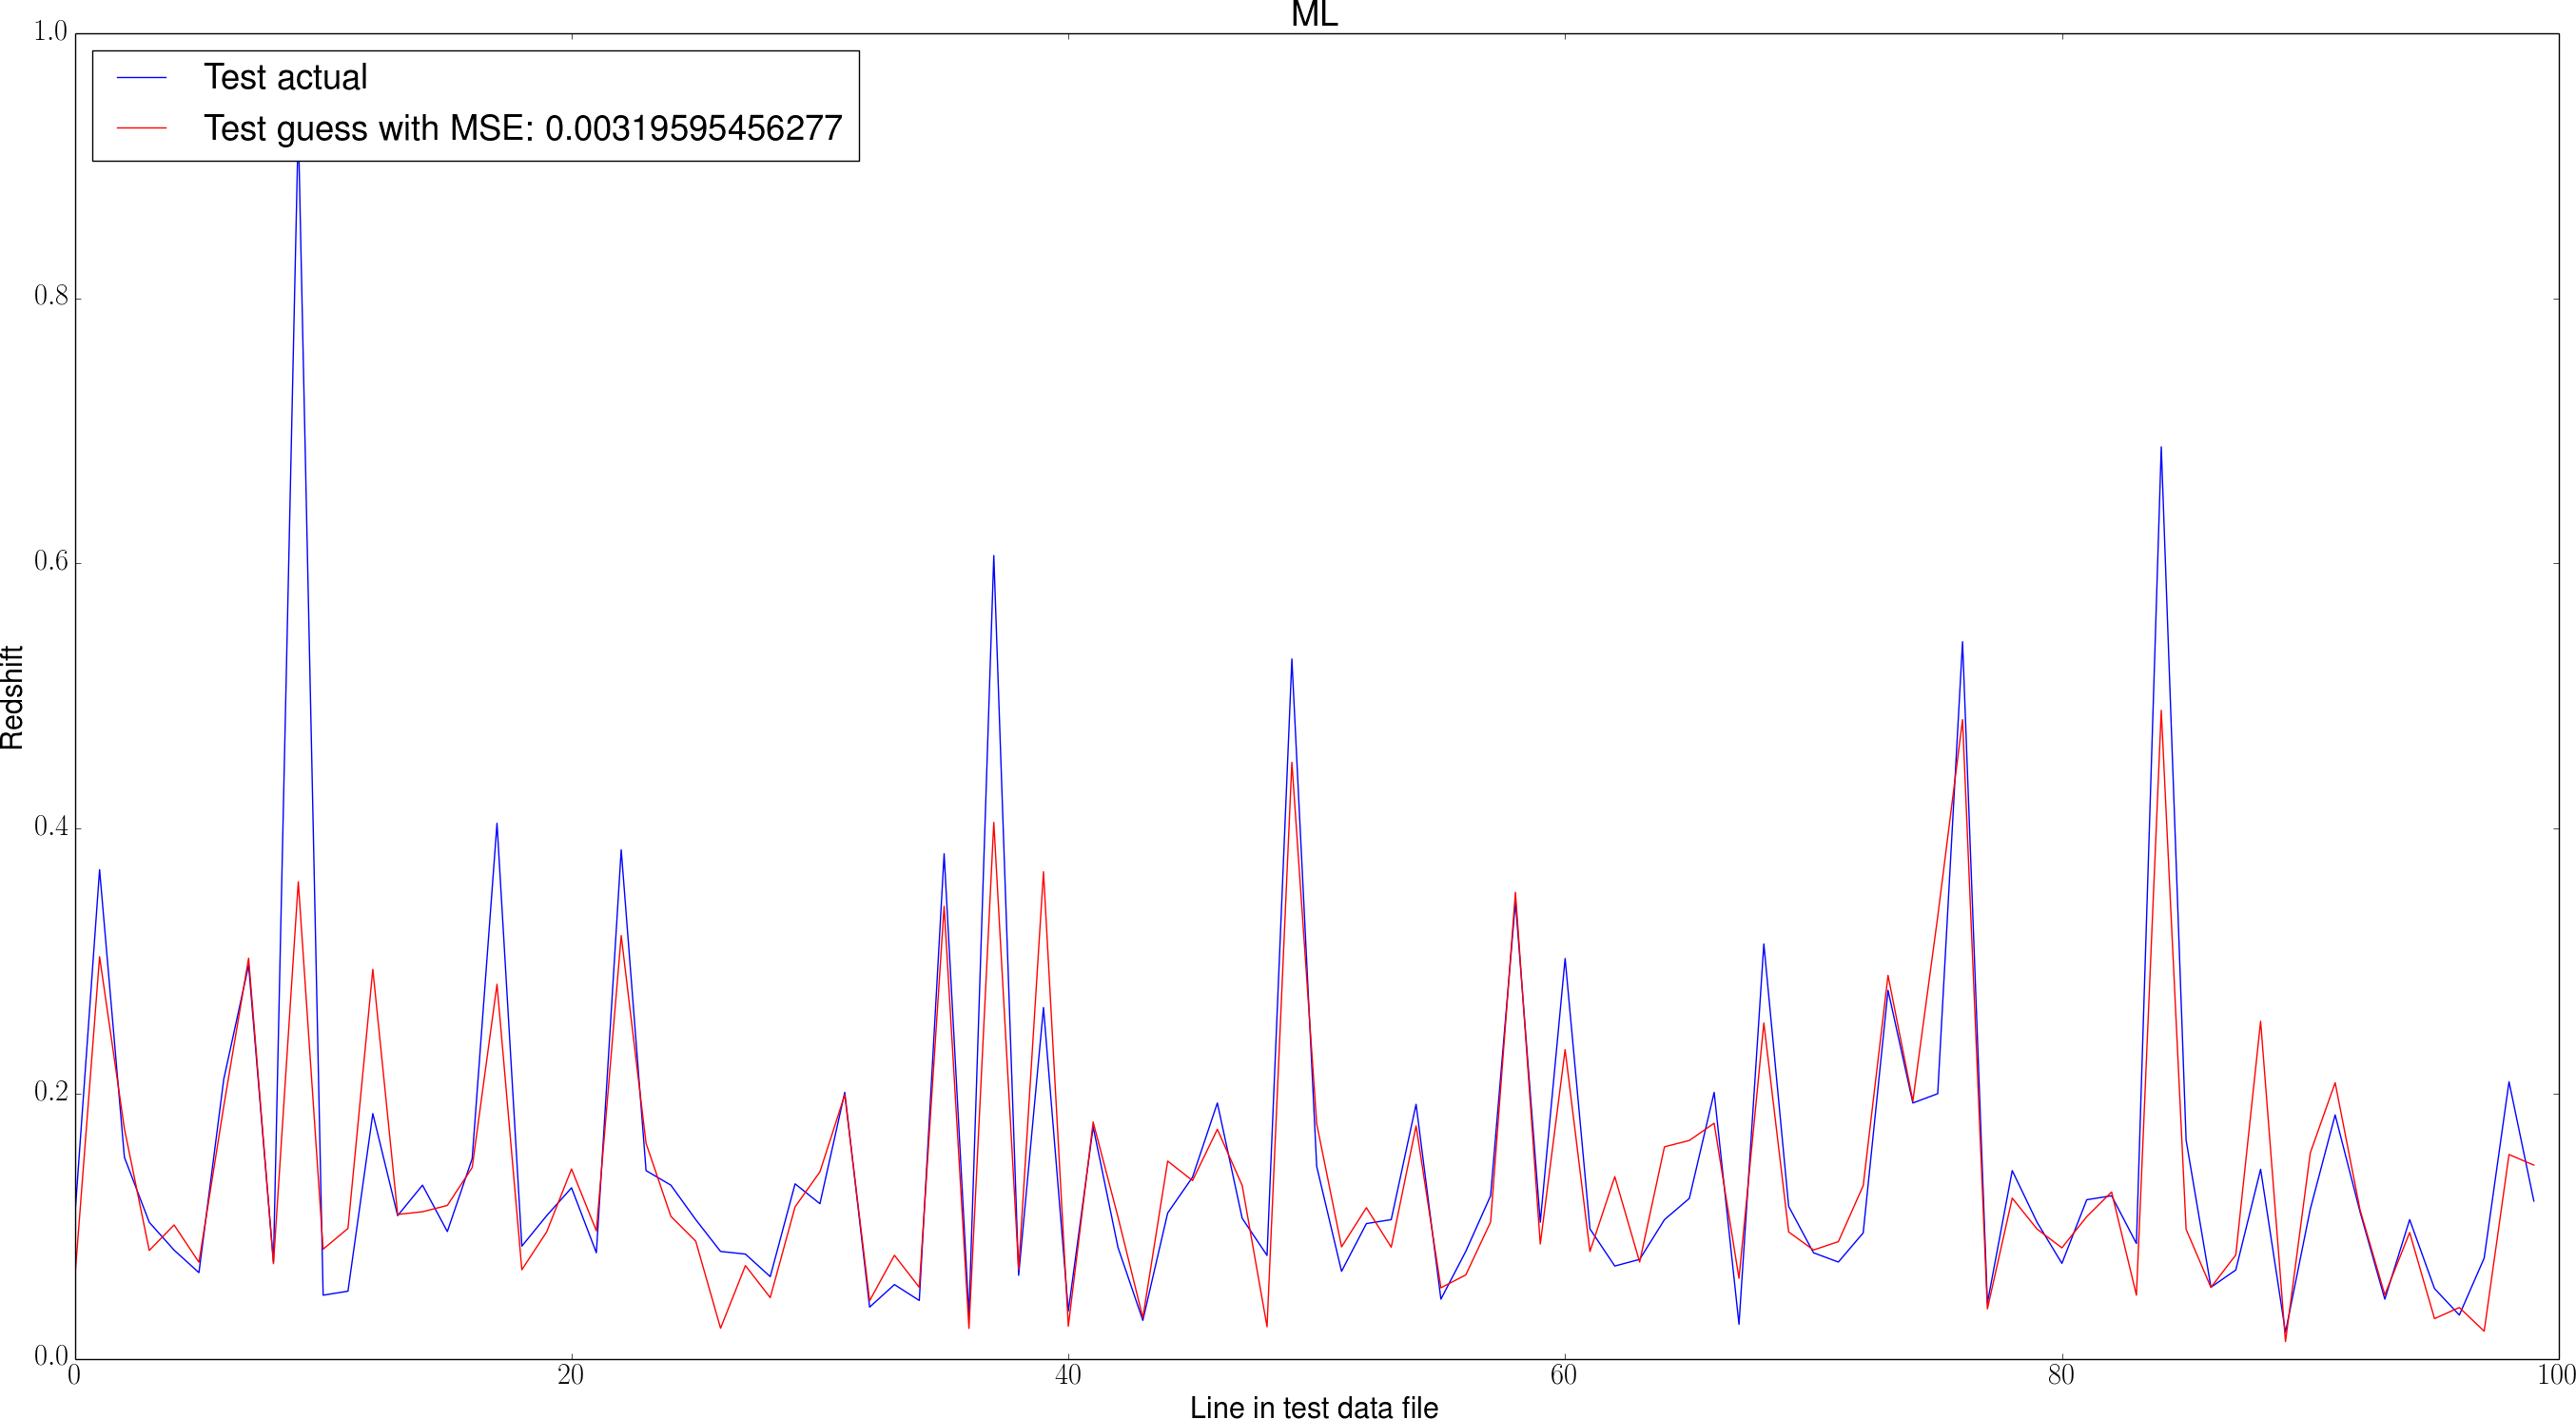
\includegraphics[scale=0.23]{linear_model_ml.png}
%	\caption{ML model measured against the test data, for the first 100 test data points.}
%	\label{fig:ml_regression}
%\end{figure}

\subsubsection{MAP results}

Through grid-search we found the best $\alpha$ to be $0$, and the best $\beta$ to be $1$. \\
We searched $\beta$ from 1 to 100, and $\alpha$ from 0 to 1 with a step of 0.01.

\begin{itemize}
	\item Training mean-squared error: $0.00281098722063$
	\item Test mean-squared error: $0.00319595456278$
\end{itemize}

\noindent As expected, we find our MSE for MAP to be equal to our MSE for ML, since our $\alpha$ is $0$.

%\begin{figure}[H]
%	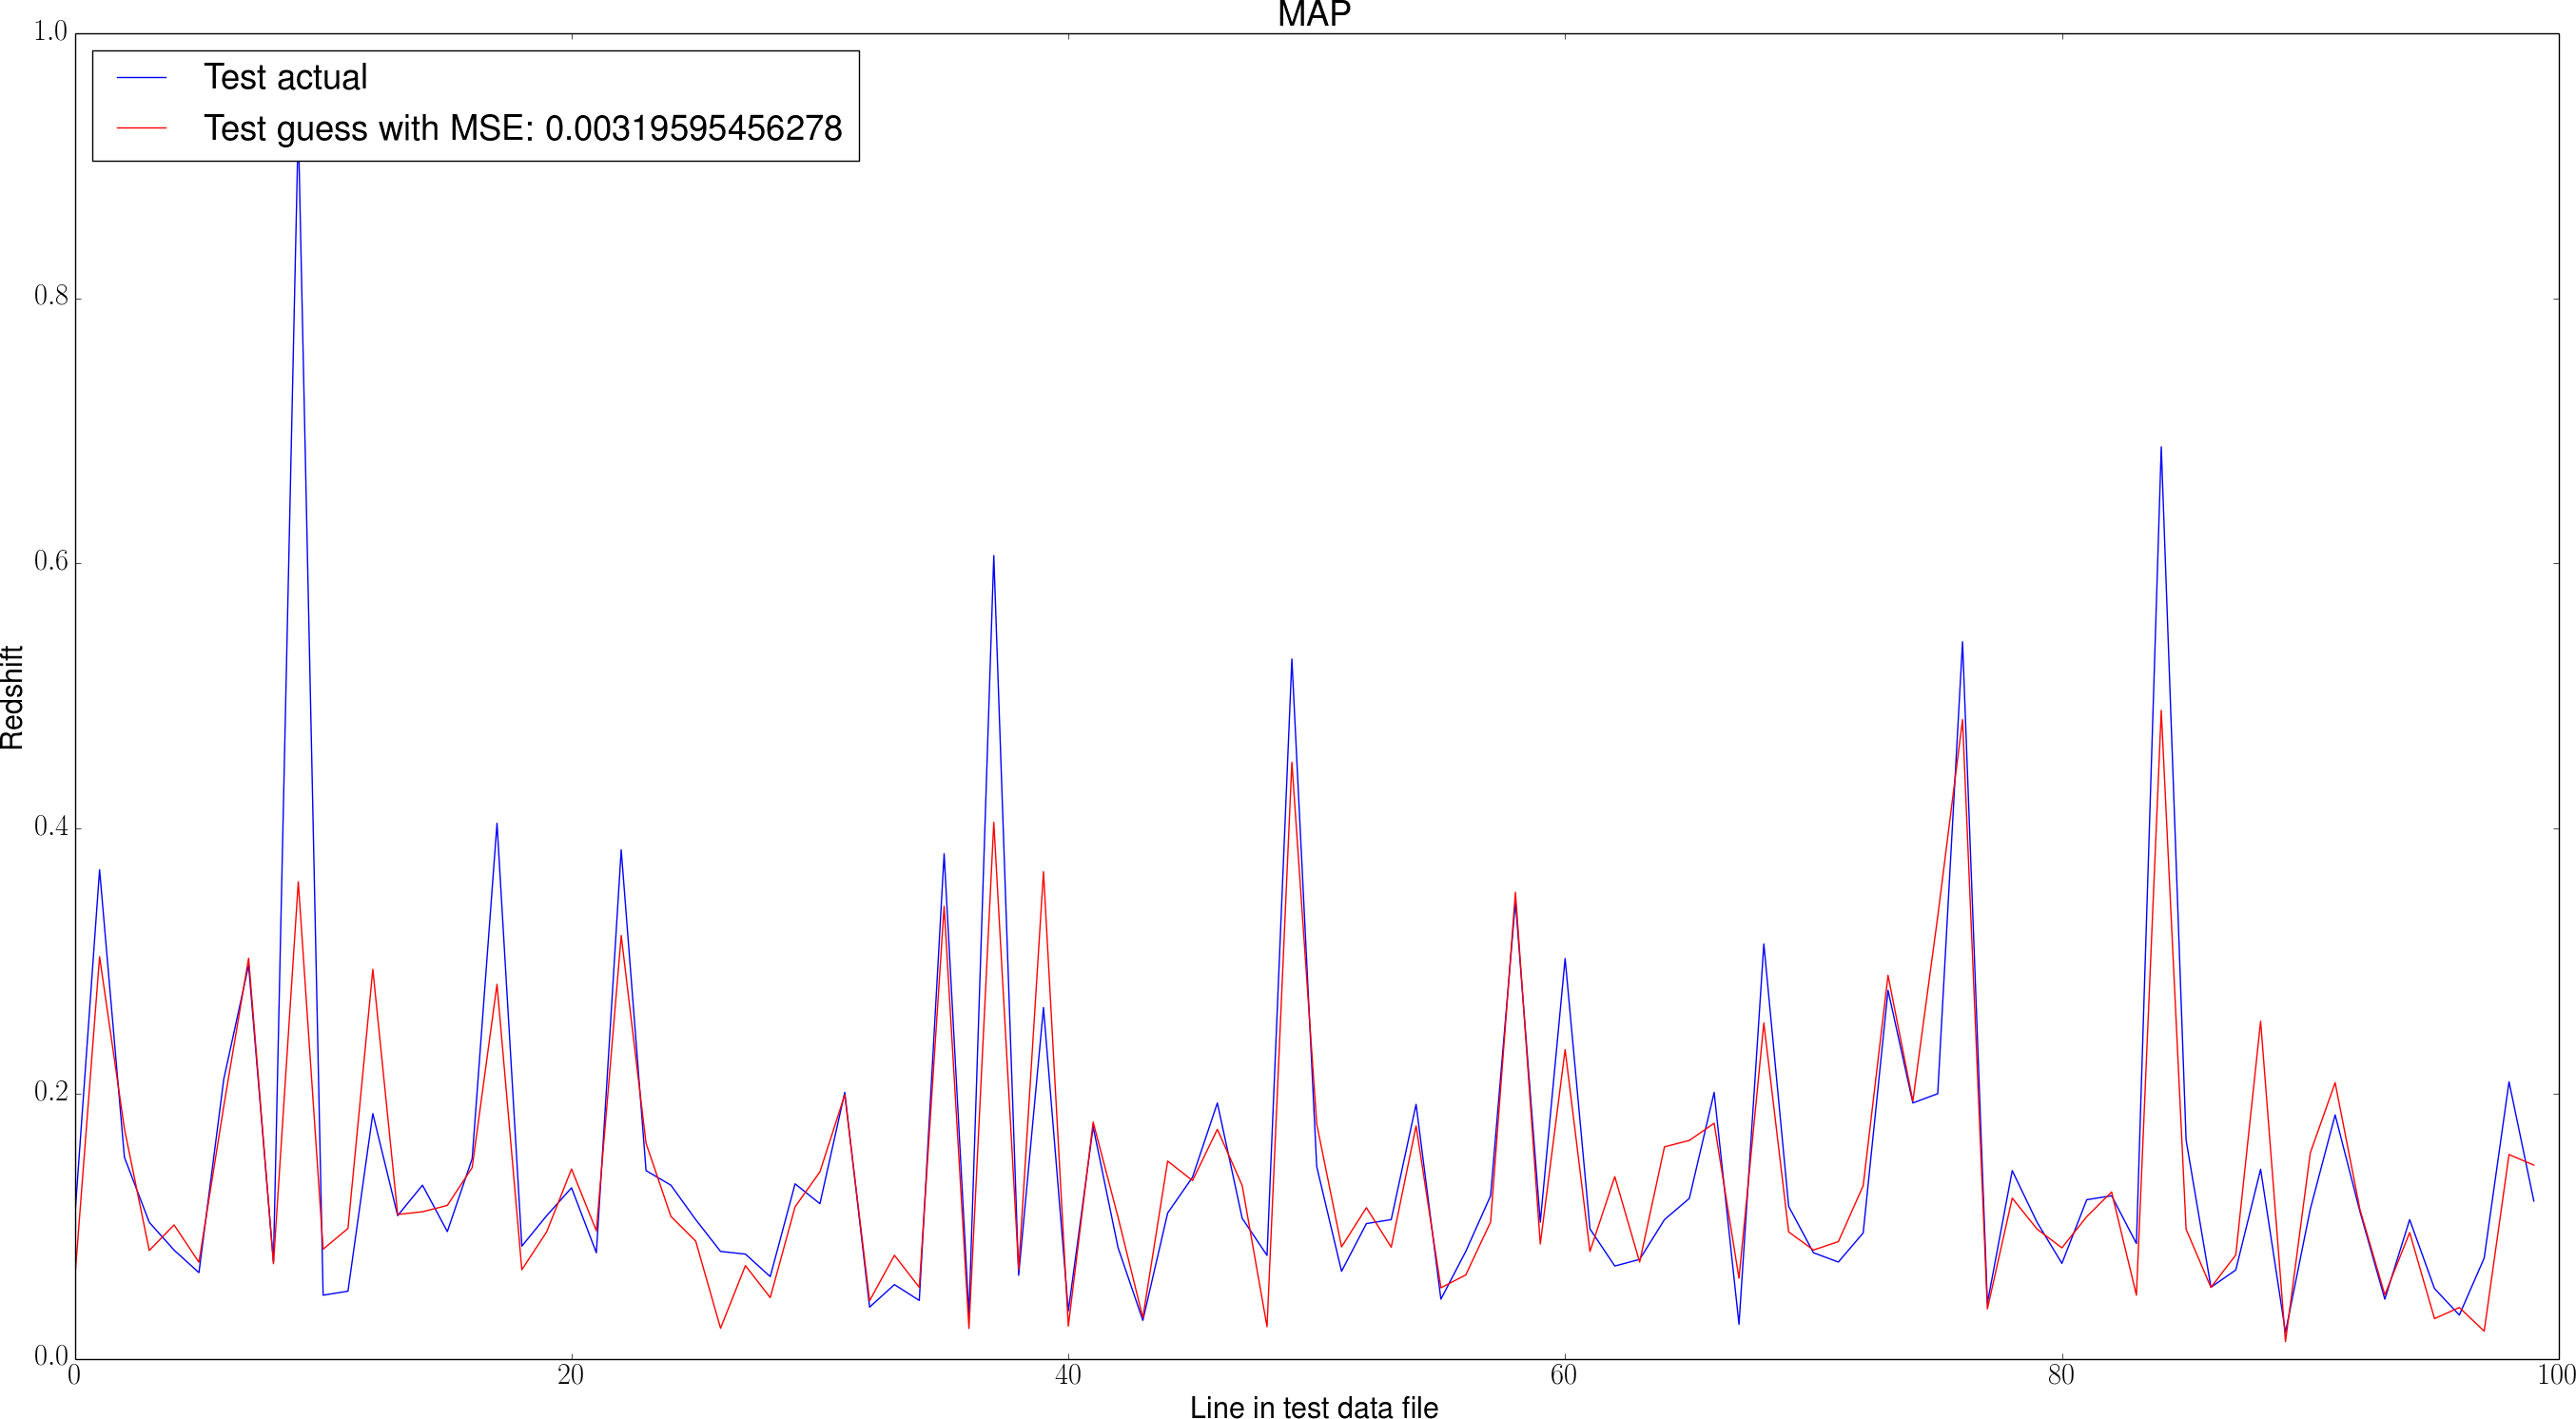
\includegraphics[scale=0.23]{linear_model_map.png}
%	\caption{MAP model measured against the test data, for the first 100 test data points.}
%	\label{fig:map_regression}
%\end{figure}

\subsubsection{SVR linear kernel results}
\label{section:SVR linear kernel results}

To discover the best parameters for SVR with linear kernel we used cross validation on $\gamma$ and $C$. We searched through $\gamma$ and $C$ incrementing by an order of magnitude in range $[-3, 3]$, starting with $\gamma$ and $C$ values of $0.1$ and $10$ respectively.

\begin{figure}[H]
	\begin{lstlisting}
	gammas = [0.1*10**i for i in range(-3, 4)]
	cs = [10*10**i for i in range(-3, 4)]
	\end{lstlisting}
	\caption{Range of $\gamma$ and $C$ to use for cross validation.}
	\label{fig:gamme_c}
\end{figure}

\noindent We found the best $\gamma$ to be 0.0001 and best $C$ to be 100.

\begin{itemize}
	\item Training mean-squared error: $0.00293831151397$
	\item Training mean-squared error: $0.00325510767138$
\end{itemize}

%\begin{figure}[H]
%	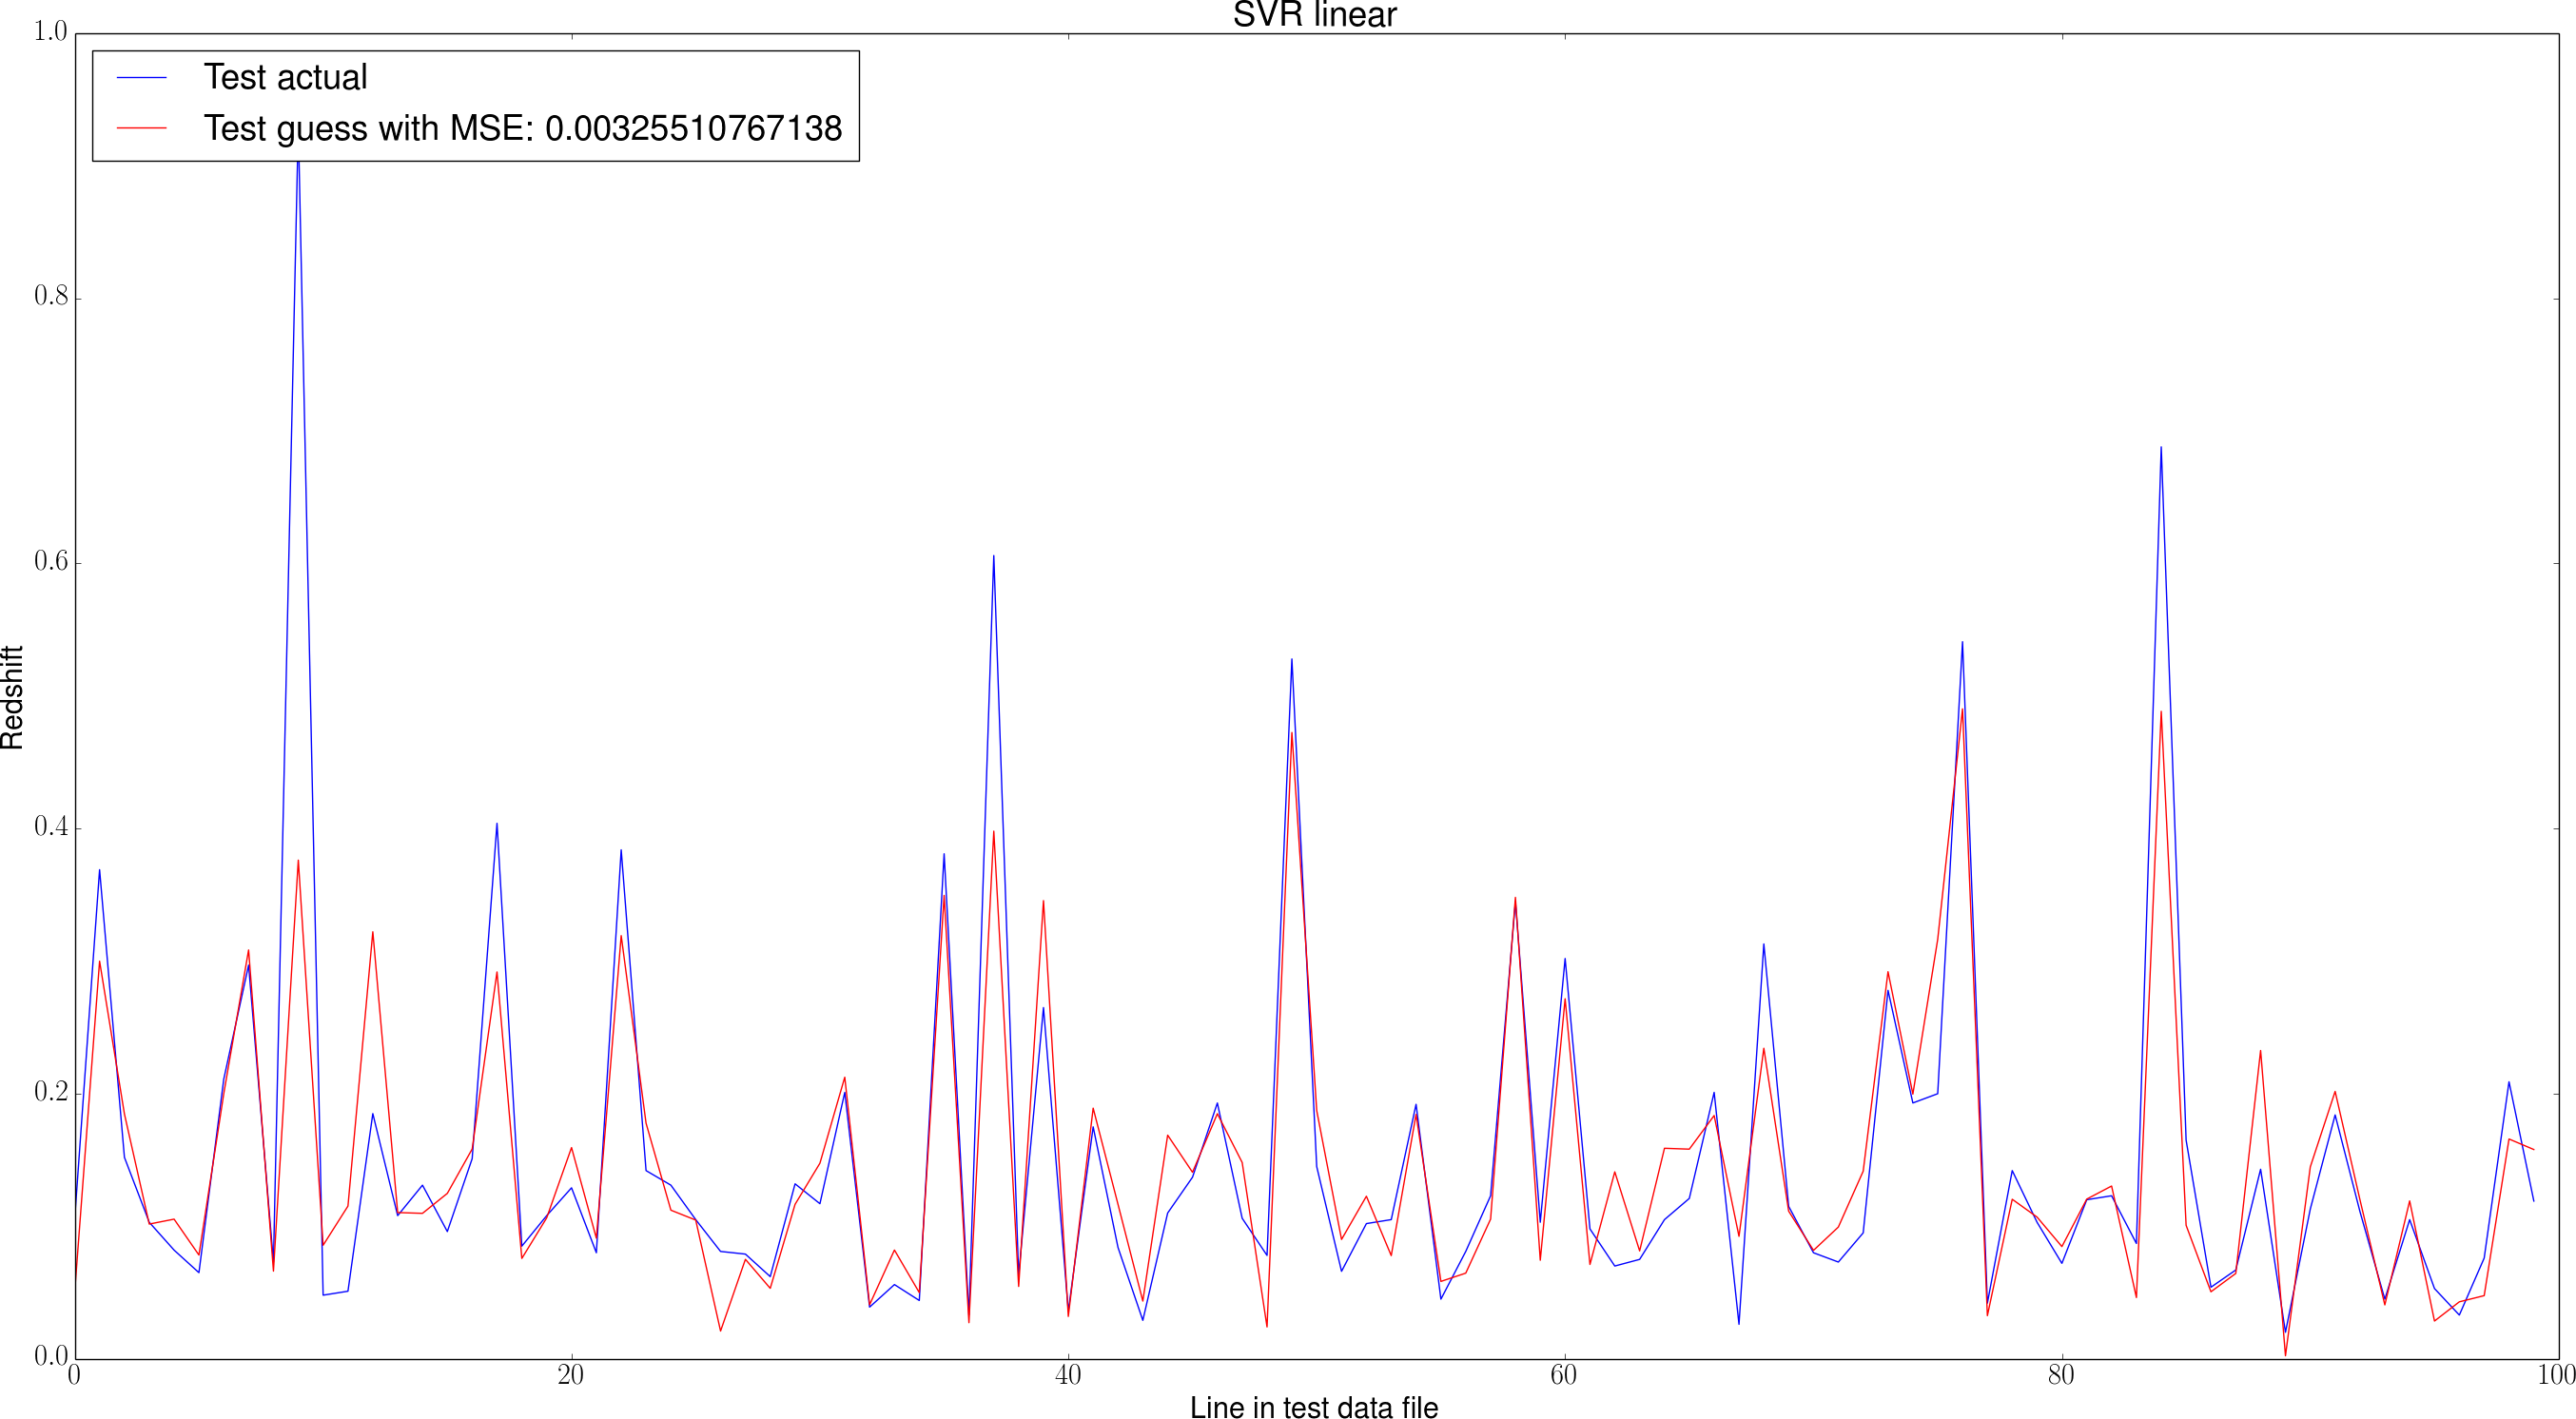
\includegraphics[scale=0.23]{linear_model_svr_linear.png}
%	\caption{SVR linear kernel model measured against the test data, for the first 100 test data points.}
%	\label{fig:svr_linear_regression}
%\end{figure}

\newpage

\subsection{Question 2 - Non-linear Regression}

For non-linear regression we decided to use Support Vector Regression with a Radial Basis Function (RBF) kernel and an polynomial kernel. \\

\noindent Again we compute and compare the MSE of our results, in order to determine the performance of our non-linear models. \\

\noindent In order to find the parameters for SVR, we performed cross validation on $\gamma$ and $C$ in the same manner as in section \ref{section:SVR linear kernel results}.
We found the best $\gamma$ to be 0.01 and the best $C$ to be 10.\\

\noindent It is worth noting that we are using the same $\gamma$ and $C$ parameters for the polynomial kernel, as for the RBF kernel. This is due to the fact that we did not get a cross validation result for the polynomial kernel, even after five hours of runtime.
We still decided to use the $\gamma$ and $C$ found for RBF, since they provided better results than the default $\gamma$ and $C$ values for the polynomial kernel. \\

\noindent As shown by the MSE of $0.00295284171625$, we actually find that Support Vector Regression with a Radial Basis Function kernel outperforms our Maximum Likelyhood approach (although very slightly).

\subsubsection{SVR RBF kernel results}

\begin{itemize}
	\item SVR rbf mean-squared training error: $0.00227026743696$
	\item SVR rbf mean-squared test error: $0.00295284171625$ 
\end{itemize}

\subsubsection{SVR Polynomial kernel results}

\begin{itemize}
	\item SVR polynomial mean-squared training error: $0.00267447888801$
	\item SVR polynomial mean-squared test error: $0.00426904768726$
\end{itemize}

\begin{figure}[H]
	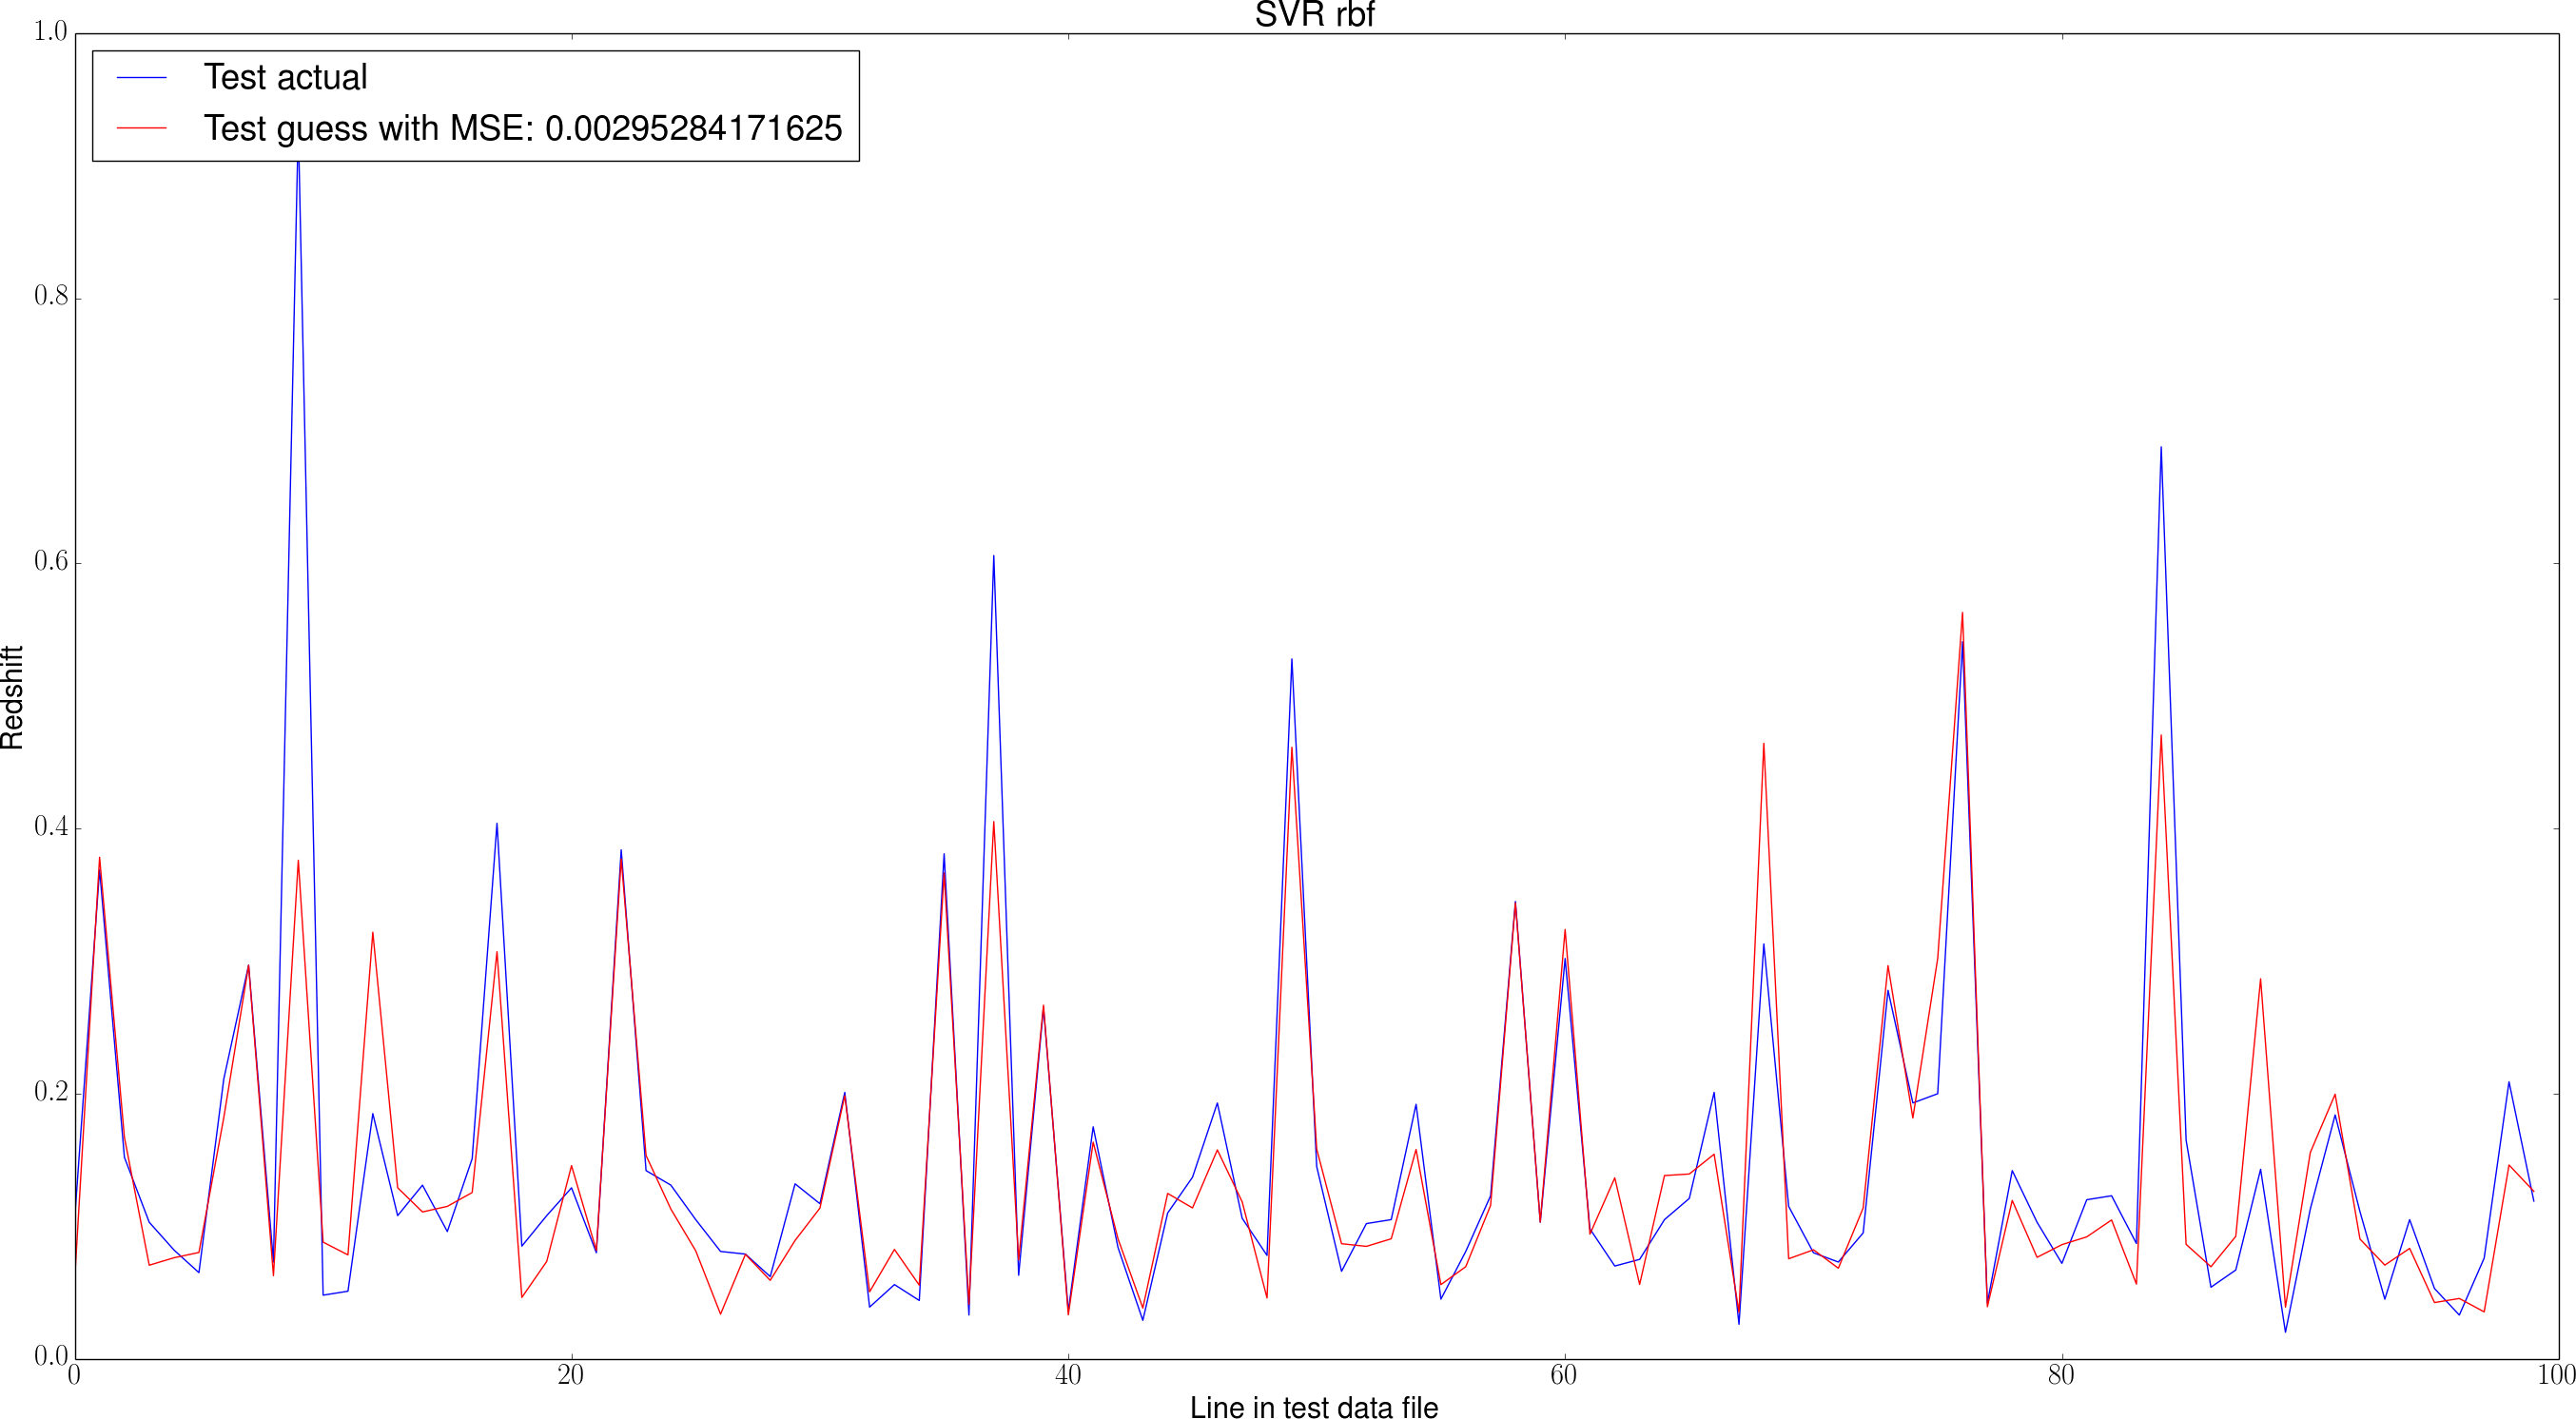
\includegraphics[scale=0.23]{linear_model_svr_rbf.png}
	\caption{SVR rbf kernel model measured against the test data, for the first 100 test data points.}
	\label{fig:svr_linear_regression}
\end{figure}

\begin{figure}[H]
	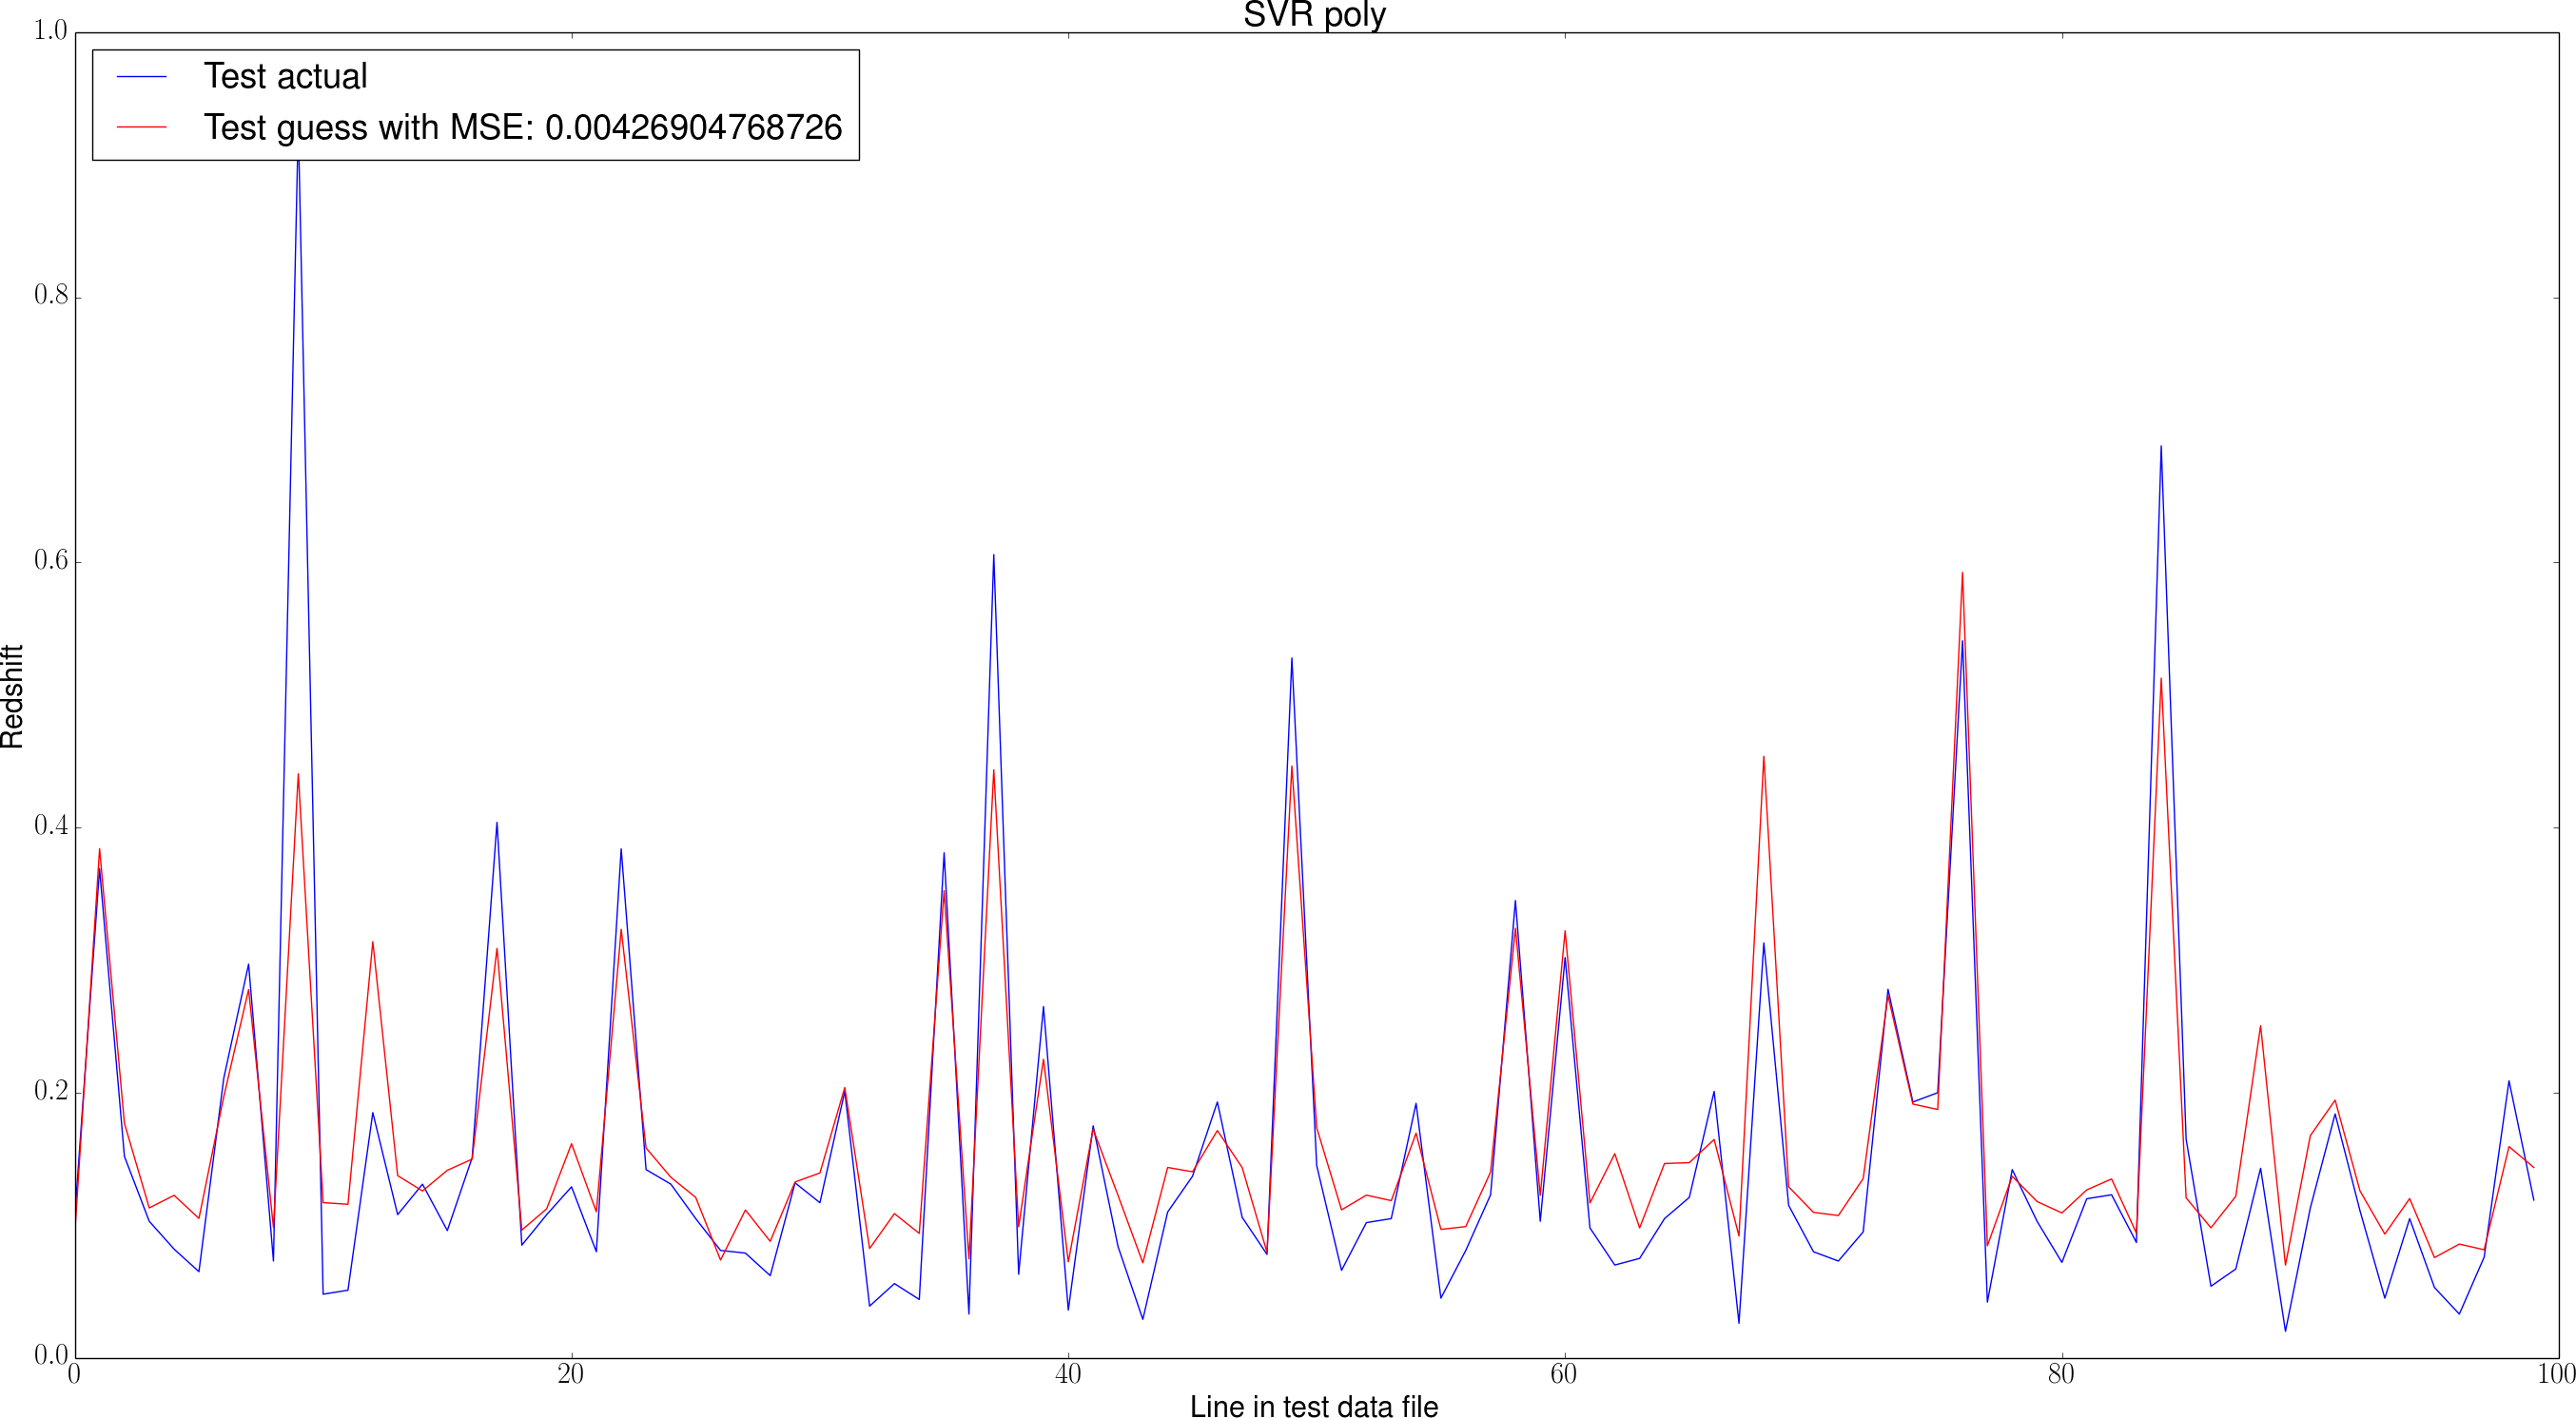
\includegraphics[scale=0.23]{linear_model_svr_poly.png}
	\caption{SVR polynomial kernel model measured against the test data, for the first 100 test data points.}
	\label{fig:svr_linear_regression}
\end{figure}

%\begin{figure}[H]
%	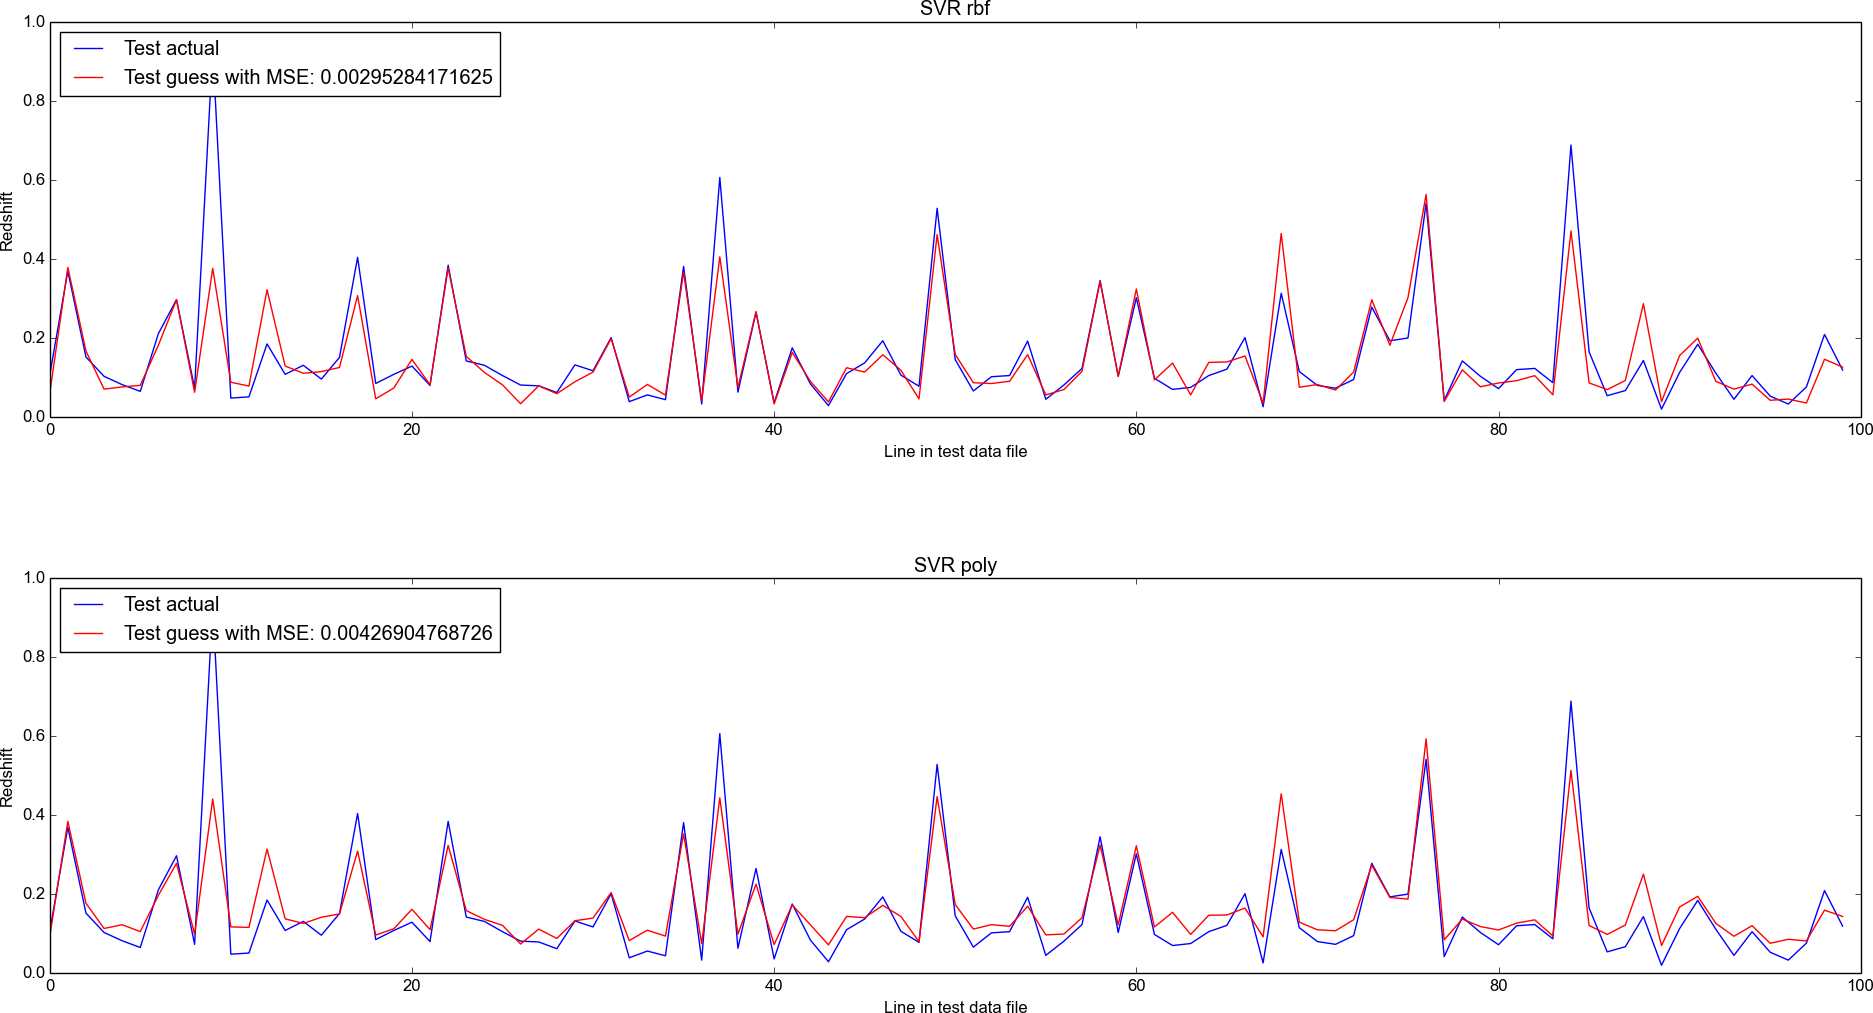
\includegraphics[scale=0.36]{nonlinear_model.png}
%	\caption{Chosen non-linear models - SVR RBF Kernel (Top), SVR Polynomial Kernel (Bottom).}
%	\label{fig:non_linear_regression}
%\end{figure}

\newpage

\subsection{Question 7 - Overfitting}

In the case of photometric redshift
estimation, we found that the following overfitting problems would be likely to apply.

\begin{enumerate}
	\item \textit{Traditional overfitting}: Train a complex predictor on too-few examples. \\
		In the case of redshift estimation we are modelling based on 10 parameters, with 2500 training samples. If we had only a hundred or a few hundred samples, such a complex predictor might have been easily overfitted in a model with several degrees of freedom.
	
	\item \textit{Parameter tweak overfitting}: Use a learning algorithm with many parameters. Choose the parameters based on the test set performance.\\
		In any case it is a common mistake to mix test and training data while building the model, and is likely to cause overfitting. \\
		In our case we are choosing our parameters for Support Vector Regression on the training set with $k$-fold cross validation on the training set.
		
	\item \textit{Brittle measures}: leave-one-out cross validation \\
		In the case of our Support Vector Regression, we used $k$-fold cross validation to choose our model parameters $\gamma$ and $C$. There might have been a chance of overfitting the $\gamma$ and $C$ parameters during cross validation, had we used leave-one-out cross validation. This might have introduced a bias in our model towards a subset of our training set.
		
		It does not seem as if the parameters for our Radial Basis Function kernel SVR model were biased. In both the case of training and test data mean-squared-error, the model performed just slightly better than Maximum Likelyhood.
		
\end{enumerate}

\newpage

\section{Cybercrime Detection}

\subsection{Question 3 - Binary Classification}

For binary classification we chose to use Linear Discriminant Analysis as our linear model, and K-Nearest Neighbour classification as our non-linear model.

\subsubsection{LDA results}

\begin{itemize}
	\item Training accuracy for LDA: 0.9921875
	\item Test accuracy for LDA: 0.9875
\end{itemize}

\noindent For training and test sensitivity and specificity we got the following results for our LDA model.

\begin{itemize}
	\item Training
		\begin{itemize}
			\item Sensitivity: 0.990625 % More good-guy classifications
			\item Specificity: 0.99375 % More bad-guy classifications
		\end{itemize}
	\item Test
		\begin{itemize}
			\item Sensitivity: 1.0
			\item Specificity: 0.975
		\end{itemize}
\end{itemize}

\noindent We see that for the test-set we are able to classify all of the good-guys correctly, whereas we are unable to correctly classify all of the bad-guys. Since we most likely could not always classify both correctly, this is our best-case scenario. We do not wish to classify good-guys as bad-guys, since we would then anger our legitimate customers. \\
Classifying a few bad-guys as good-guys is much better, since we might be able to use other measures to further prevent them from doing bad-guy stuff.

\newpage

\subsubsection{KNN results}
\label{section:binary classification - knn}

For our KNN classifier we ran cross validation in order to discover the best $k$. We used a fold of 5 and a $max_k$ of 25. We found the best $k$ to be 1.

\begin{itemize}
	\item Training accuracy for KNN: 1.0
	\item Test accuracy for KNN: 0.98125
\end{itemize}

\noindent For training and test sensitivity and specificity we got the following results for our 1-NN model.

\begin{itemize}
	\item Training
		\begin{itemize}
			\item Sensitivity: 1.0
			\item Specificity: 1.0
		\end{itemize}
	\item Test
		\begin{itemize}
			\item Sensitivity: 0.9875
			\item Specificity: 0.975
		\end{itemize}
\end{itemize}

\noindent We are able to classify good-guys slightly worse than with our LDA classifier, and classify bad-guys with the same precision. This makes KNN slightly less preferable to our LDA model, since we with KNN are going to exclude some legitimate customers from our service.

\newpage

\subsection{Question 4 - Principal Component Analysis}

In order to compute the eigenvalues and eigenvectors we used the numpy.linalg.eig library. We then use the eigenvectors with the smallest eigenvalues to define $W$ and then scale our datapoints accordingly.

\begin{figure}[H]
	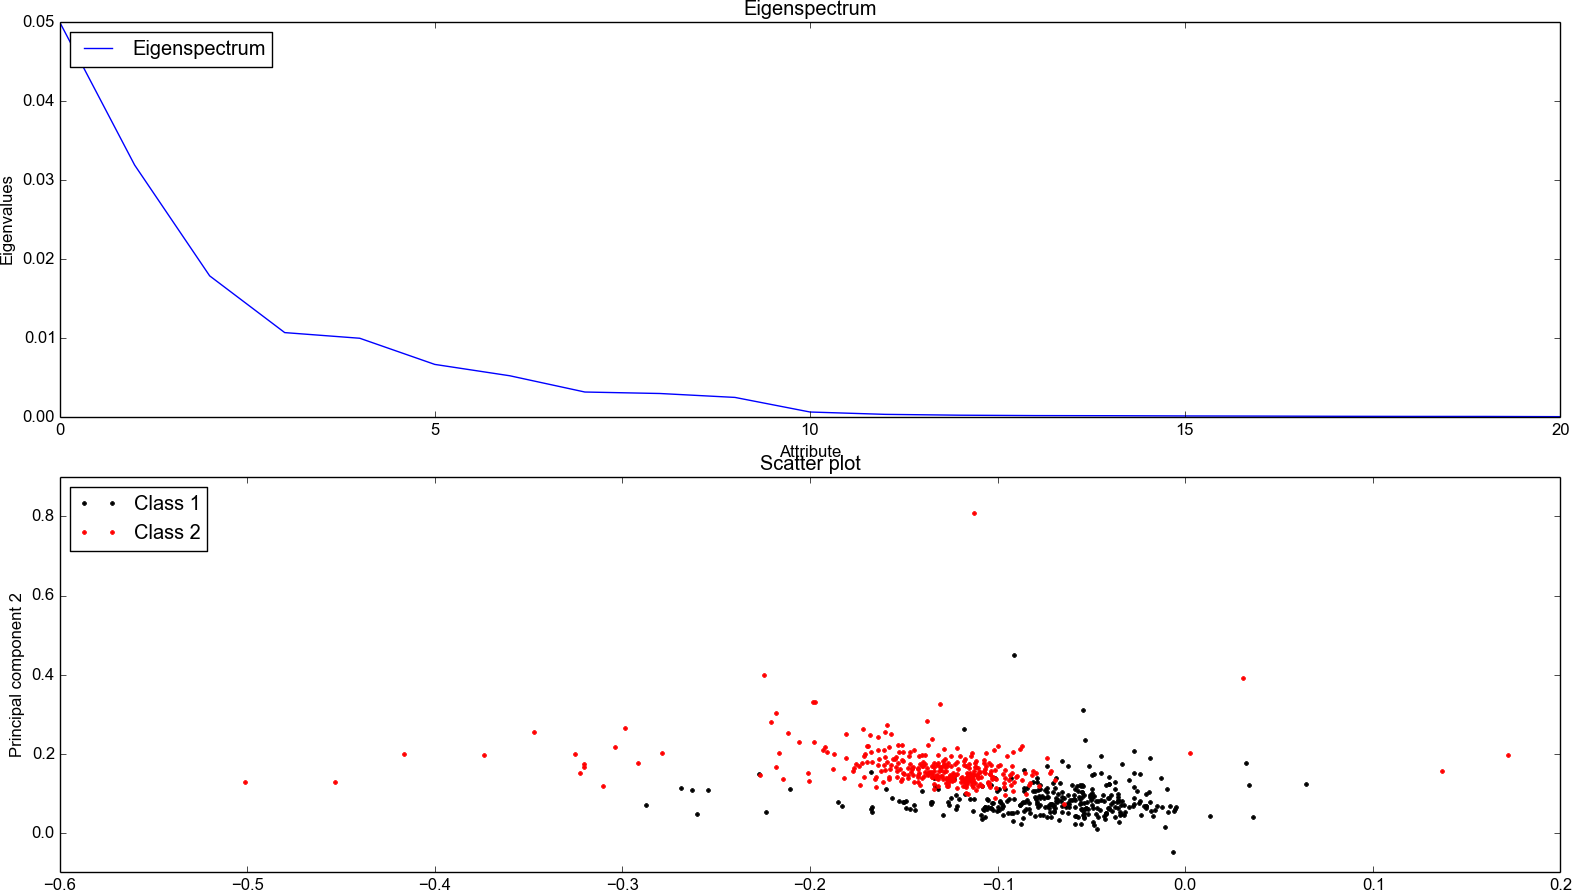
\includegraphics[scale=0.45]{principal_component_analysis.png}
	\caption{Eigenspectrum for all components (Top). Principal components coloured by class (Bottom).}
	\label{fig:svr_linear_regression}
\end{figure}

\newpage

\subsection{Question 5 - Clustering}

We notice that the cluster centers fit quite well with the two classes. In order to find the centers we used the same approach as with PCA.

\begin{figure}[H]
	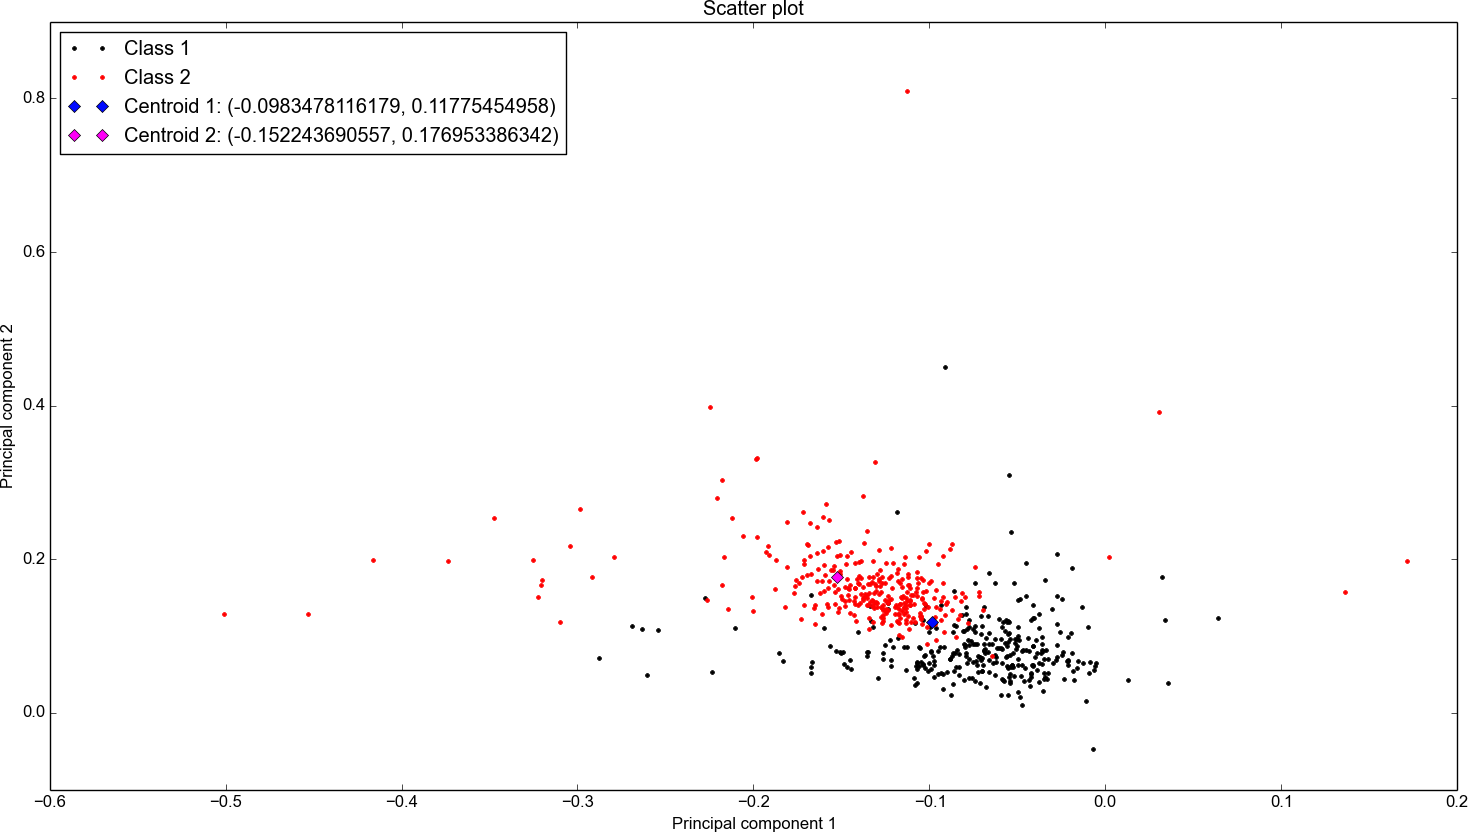
\includegraphics[scale=0.45]{principal_component_analysis_centroids.png}
	\caption{Principal components coloured by class along with the two cluster centers.}
	\label{fig:svr_linear_regression}
\end{figure}

\newpage

\subsection{Question 6 - Multi-Class classification}

We used K-Nearest-Neighbour and Linear Discriminant Analysis as our models, since we had already implemented support for higher dimensions during the course assignments.
In order to determine the best $k$ we used the same cross validation approach as in section \ref{section:binary classification - knn}.\\

\noindent The implementations used for both LDA and KNN was our own from the course exercises, which rely on the python numpy library for matrix operations, and on the python scipy library for calculating distances between points in higher dimensions for K-Nearest-Neighbour.\\

\noindent KNN classifier best k:1 \\
KNN training accuracy: 1.0 \\
KNN test accuracy: 0.9075 \\

\noindent Training accuracy for LDA: 0.928125 \\
Test accuracy for LDA: 0.9175 \\

\noindent These results are slightly worse than our binary classification results, but considering the fact that we can classify 4 classes instead of 2, it is most likely also more useful. 

\end{document}
